%%%%%%%%%%%%%%%%%%%%%%%%%%%%%%%%%%%%%%%%%%%%%%%%%%%%%%%%%%%%%%%%%%%%
% Grundlagen
%%%%%%%%%%%%%%%%%%%%%%%%%%%%%%%%%%%%%%%%%%%%%%%%%%%%%%%%%%%%%%%%%%%%

\chapter{Principles}
  \label{Principles}

\section{Trello}

\subsection{How Trello works}\index{Trello}
Trello is a webservice by the New York City based web corporation Fog Creek Software\footnote{Official Fog Creek Software website: \url{http://www.fogcreek.com}}\index{Fog Creek Software}. It is a collaboration tool to manage projects, launched in 2011\footnote{The original launch post in the Trello blog: \url{http://blog.trello.com/launch/}}. 

\begin{figure}[htb]
\centering
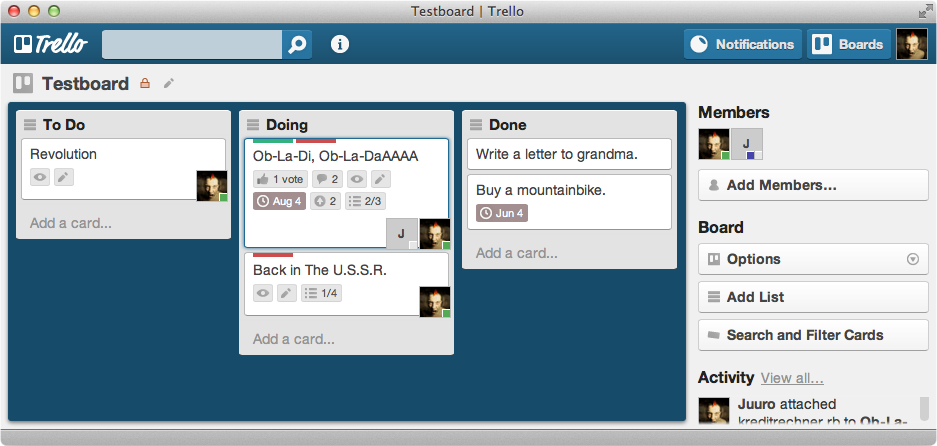
\includegraphics[width=\textwidth]{figures/trello}
\caption{A Trello board.}
\label{fig:trello}
\end{figure}

There is the concept of so called \emph{boards} which contents several configurable lists. Figure \ref{fig:trello} shows a board with the three standard lists \emph{To Do}, \emph{Doing} and \emph{Done}. In these lists the user can create todo items. These todo items are called \emph{cards}. The cards can contain several additional data. Each card has a title and maybe a description, some asigned members, a due date, some labels, votes, checklists, comments and attachments. The creator of the board is the owner in the first place and the owner can add other Trello users to his boards and cards. So everone who's working on a project can see whats going on at the moment. Users who are assigned to a board can even create new todo items by themselves. If somebody works at more than one company with many projects each there is the concept of \emph{organizations}. This is useful in order to ensure a clear separation.

\begin{figure}[htb]
\centering
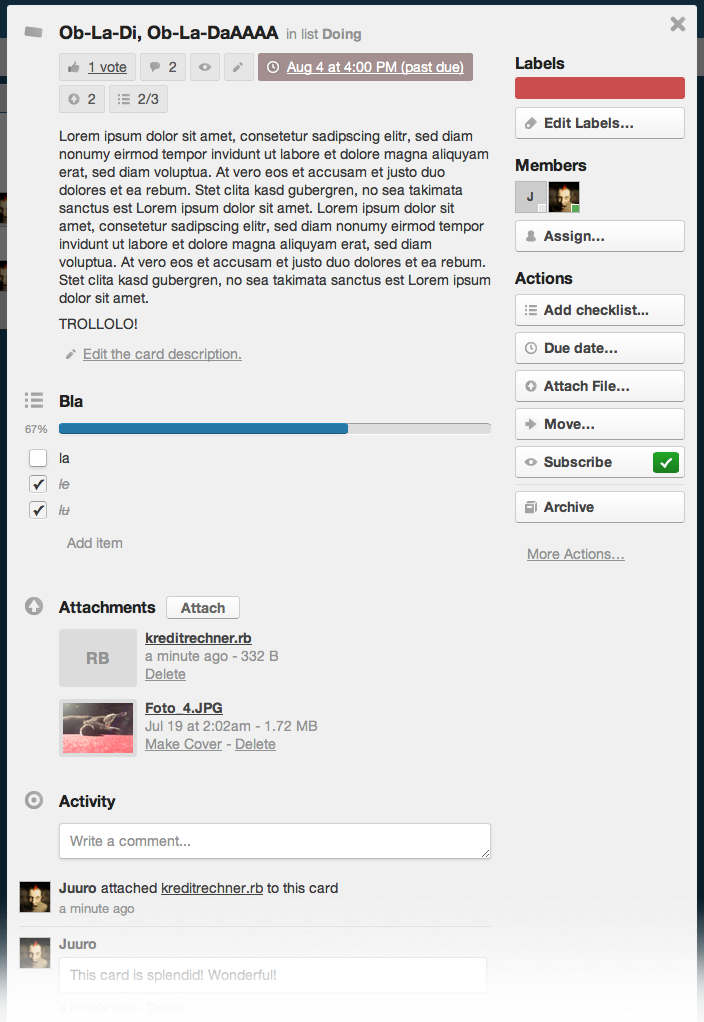
\includegraphics[width=\textwidth]{figures/trello-card}
\caption{A opened card in Trello.}
\label{fig:trello-card}
\end{figure}

\subsection{Why Trello}\index{Trello}
Trello is not just one of hundreds of thousands of todo applications. It is streamlined for the purposes of small businesses. So for the needs in the university with small groups of people working on the same things it is perfect. Trello has proofed its value several months already. The Trello website is written in HTML 5\index{HTML!5} with the use of AJAX\index{AJAX} where it makes sense. Trello provides an iOS\index{iOS} \cite{trello:ios} and Android\index{Android} \cite{trello:android} app. Both are constantly evolving. So the system is state-of-the-art. In addition the company behind Trello is not just a start-up with three employees. Thats important, too. A product of a small business, which is based just on the enthusiasm of the founders often doesn't last long. Fog Creek Software is over ten years old and has several products.

The first wish was to see the due dates of the cards anybody is assigned to in Google Calendar. But thinking about that there were many other use cases for small scripts which could run as cron jobs on a server to serve several regular tasks. These scripts are described in more detail in Chapter 3.

\subsection{Trello API}\index{API}
Trello has an API \nomenclature{API}{Application Programming Interface} which is still in beta at the moment I'm writing this. But it is already very extensive. \cite{trello:docu}

\subsubsection{REST}\nomenclature{REST}{Representational State Transfer}
The Trello API is a \emph{RESTful} web API. That means that the API is conform to the REST design model. REST is a common style of software architecture for distributed systems. An implementation of a REST web service follows four basic design principles:
\begin{itemize}
	\item Use HTTP\nomenclature{HTTP}{Hyper Text Transfer Protocol} methods explicitly.
	\item Be stateless.
	\item Expose directory structure-like URIs\nomenclature{URI}{Uniform resource identifier}.
	\item Transfer XML\nomenclature{XML}{Extensible Markup Language}, JSON\nomenclature{JSON}{JavaScript Object Notation}, or both.
\end{itemize}

\cite{rest}

\subsubsection{Authentification}
Though the scripts which are used here need access to private boards in Trello\index{Trello} there has to be any kind of authentification. For user applications with a frontend the Trello API provides OAuth2. But because of the concept of OAuth2 the user is required to enter his Trello username and password. \cite{oauth} My scripts are supposed to run on servers as cron jobs. There is no user who could manually enter data. For this kind of applications Trello provides a key/token-system. Every user has a private key. Whith this key the user can generate a token. This token will be send along every request to the Trello API. The token tells Trello which scope the request can see. While generating a token one can specify the scope of the token and when it will expire. The possible expriations of a token are between one day and never. In our case we will use \emph{never}. To generate a token one has to visit a special URL:
\texttt{
https://trello.com/1/authorize?key=SUBSTITUTEWITHYOURPRIVATEKEY \&name=My+Application\&expiration=never\&response\_type=token \&scope=read,write}
In this example the token would never expire and could read and write everything the user can access with the API. Other valid values instead of \texttt{never} for expiration would be \texttt{1day}, \texttt{30days}. \texttt{30days} is the default value. \cite{trello:gettingstarted}

\section{JSON}\index{JSON}
All the responses to Trello\index{Trello} API\index{API} calls use JSON. It is a subset of the JavaScript programming language. Despite its relation to JavaScript it's language independent. JSON is da data-interchange format like XML\nomenclature{XML}{Extensible Markup Language}. But JSON is built on two structures. One is a list of key/value pairs. In most programming languages this is realised as an hash, struct, object or associative array. The other structure is an ordered list of values. This is realised as array, list, vector or sequence in popular programming languages. In JSON itself these structures are called \emph{object} and \emph{array}. Objects start and end with braces. Each key is followed by a colon and the key/value pairs are separated by commas. Arrays start and end with brackets. The values are separated by commas. Both can be arbitrary nested. At every point one of my script saves content at any other place than Trello it's in the JSON\index{JSON} format, too. That's because it guarantees easy compatibility with Trello. JSON\index{JSON} can be saved in files, too. A JSON\index{JSON} file has the suffix \texttt{.json}. \cite{json}

\section{Ruby}\index{Ruby}
Ruby is a modern general-purpose object-oriented programming language. Its big difference to most other languages is that it focuses on humans rather than computers. 

Yukihiro Matsumoto, the designer of Ruby, said once:
\begin{quote}
Ruby is simple in appearance, but is very
complex inside, just like our human body.\cite{ruby:talk}
\end{quote}

That means, that Ruby\index{Ruby} is very easy readable and is intuitive for humans even so it can perform complex tasks. This is achieved with English keywords instead of brackets and braces. The result for the programmer of this consistent philosophy is a very easy to read language which is also very plain. Because of the English words instead of abstract characters Ruby is easy understandable. Even non-programmers understand mostly whats going on. So programmers produce way less errors while writing the code. A wrongly spelled word is more intuitive recognisable than a missing bracket or semicolon. \cite{ruby:about} More about Ruby can be found at \url{http://www.ruby-lang.org}.

\subsection{RubyGems}\index{RubyGems}
Ruby has a good amount of methods and classes every Ruby installation provides. But there are hundreds of extensions for special use cases – to communicate with RESTful Web APIs for example – made by third party developers. In Ruby such extensions are called \emph{gems}. To manage and publish these third party libraries theres is the standard \emph{RubyGems}. It provides a standard format for third party libraries for Ruby, a tool to manage the installation of gems and a server for distributing the gems. \cite{ruby:gemdev} Some Ruby distributions are delivered with several gems. Gems can be added to an existing Ruby installation at any time. 

To install an additional gem on a Unix operating system the following command can be used:  
\begin{center}
\texttt{gem install gemname}
\end{center}
Where \texttt{gemname} is the name of the respective gem. If the installation performed without errors, the gem is ready to use. \cite{ruby:gemdoc}

To use an installed gem in a Ruby\index{Ruby} script the following code at the top of the script before the code starts is necessary:

\begin{lstlisting}[float=htb, caption=Using the gem \emph{gemname}, label=listing001]
require 'gemname'
\end{lstlisting}
Again, \emph{gemname} stands for the name of the respective gem. If any gems are used in these script which are not part of the Ruby standard distribution, they are listed at the beginning of the related description. Further information at \url{http://doc.rubygems.org} and \url{http://rubyforge.org/projects/rubygems/}.

